
\subsection{\elemRowOpsTitle: Explanation of Proof for Theorem~\ref{GJEunique}}

{\ttfamily
\fontdimen2\font=0.4em
\fontdimen3\font=0.2em
\fontdimen4\font=0.1em
\fontdimen7\font=0.1em
\hyphenchar\font=`\-

\hypertarget{scripts_elementary_row_operations_proof}{The first thing to realize is that} 
there are choices in the Gaussian elimination recipe, so maybe that could lead to two different
RREF's and in turn two different solution sets for the same linear system. But that would be weird,
in fact this Theorem says that this can never happen!

Because this proof comes at the end of the section it is often glossed over, but it is a very important result.
Here's a sketch of what happens in the video:
\begin{center}
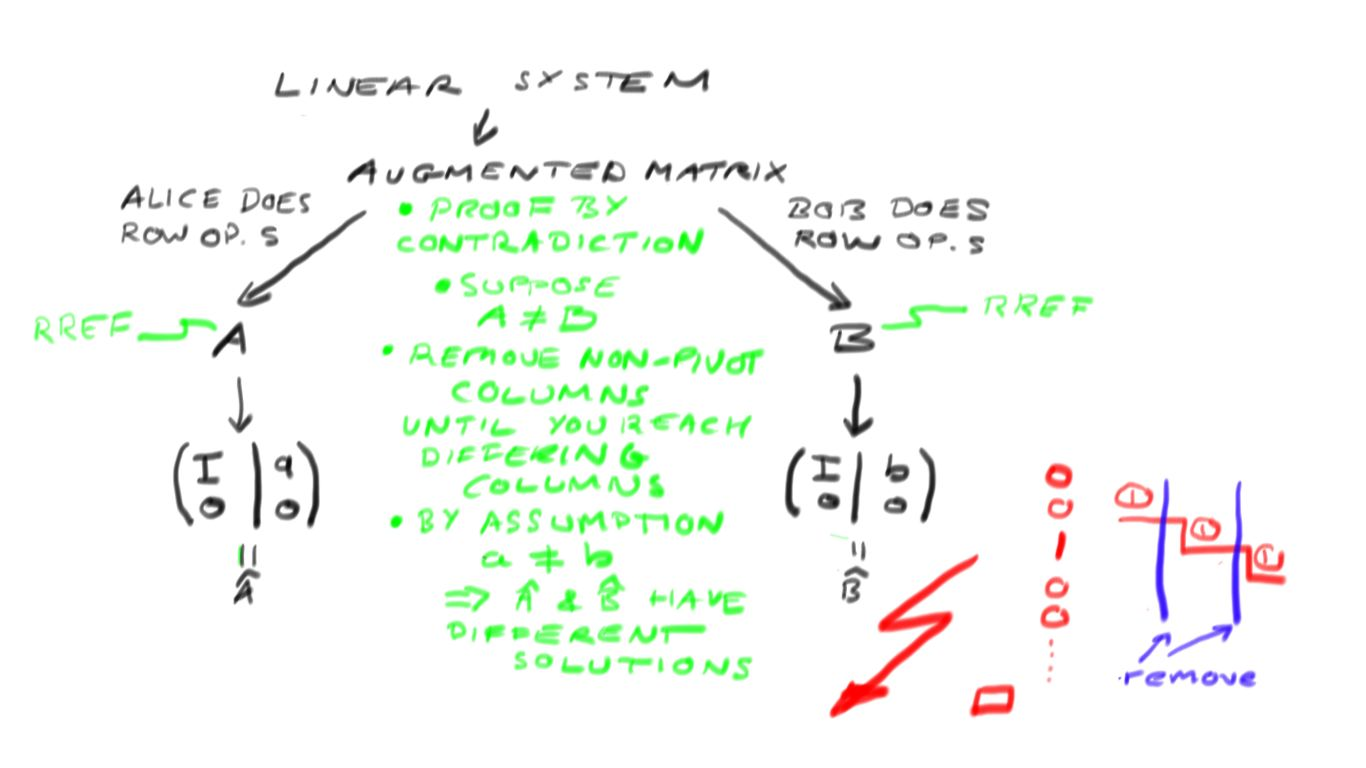
\includegraphics[scale=.3]{RREF_unique.jpg}
\end{center}

In words: we start with a linear system and convert it to an augmented matrix. Then, because we are studying a uniqueness
statement, we try a proof by contradiction. That is the  method where to show that a statement is true, you try to demonstrate that
the opposite of the statement leads to a contradiction. Here, the opposite statement to the theorem would be to find
two different RREFs for the same system.

Suppose, therefore, that Alice and Bob do find different RREF augmented matrices called $A$ and $B$. 
Then remove all the non-pivot columns  from $A$ and $B$  until you hit the first column that differs. Record that in the last column
and call the results $\widehat A$ and $\widehat B$. Removing columns
does change the solution sets, but it does not ruin row equivalence, so  $\widehat A$ and $\widehat B$ have the same solution sets.

Now, because we left only the pivot columns (plus the first column that differs) we have
$$\hat{A}=\begin{amatrix}{1}
I_N & a\\
0 & 0
\end{amatrix} \mbox{ and } \hat{B}=\begin{amatrix}{1}
I_N & b\\
0 & 0
\end{amatrix}\, ,$$ where $I_N$ is an identity matrix and $a$ and $b$ are column vectors.
Importantly, by assumption,
$$
a\neq b\, .
$$
So if we try to wrote down the solution sets for $\widehat A$ and $\widehat B$ they would be different.
But at all stages, we only performed operations that kept Alice's solution set the same as Bob's.
This is a contradiction so the proof is complete.
} % Closing brace for the font

\newpage
